\chapter{Marco teórico}
\graphicspath{{figs/}}
\label{Modelo teórico}

\section{Modelo SIR}
\label{S:Modelo SIR}

El modelo SIR describe la dinámica de tres grupos característicos de un sistema, denominados comunmente como \textbf{S}usceptibles, \textbf{I}nfectados y
\textbf{R}ecuperados, de ahí su nombre. Es el modelo más simple que puede encontrarse para describir la propagación de una enfermedad 
infecciosa. El mismo está formulado de la siguiente manera: sean $S(t)$, $I(t)$ y $R(t)$ la fracción de susceptibles, infectados
y recuperados de una población dada a tiempo $t$ respectivamente, entonces la dinámica de estos grupos está descripta por el sistema de
ecuaciones diferenciales ordinarias
\begin{align}
  \dv{S}{t}&=-\beta SI,\label{Seq}\\[.3cm]
  \dv{I}{t}&=\beta SI - \gamma I,\label{Ieq}\\[.3cm]
  \dv{R}{t}&=\gamma I.\label{Req}
\end{align}
Donde $\beta$ corresponde a una tasa de transmisión mientras que $\gamma$ corresponde a una tasa de recuperación.

Usualmente la ecuación 
para $R$ (\ref{Req}) no se escribe ya que puede ser reemplazada por la más simple $S+I+R=1$. Puede verse por inspección que el sistema de ecuaciones
(\ref{Seq} - \ref{Req}) cumple $\dv{S}{t}+\dv{I}{t}+\dv{R}{t}=0$, como corresponde.

Para entender porqué este simple sistema de ecuaciones (\ref{Seq} - \ref{Req}) gobierna la dinámica del problema observamos que el mismo 
está compuesto esencialmente por dos términos, el término de transmisión $\beta SI$ y el de recuperación $\gamma I$. Cualitativamente, resulta 
razonable que la magnitud de sujetos infectados por unidad de tiempo aumente con el producto de la cantidad de infectados y susceptibles, de ahí 
el término de transmisión. Por otro lado, la cantidad de infectados que se recuperan por unidad de tiempo es entendible que sea proporcional a la
misma cantidad de infectados y de ahí el término de recuperación. Por supuesto, es posible justificar esto de una manera más cuantitativa y precisa, para 
ver una derivación de estas ecuaciones consultese \cite{SIR,keeling:infectious_diseases}.

A pesar de su simplicidad, este modelo (\ref{Seq} - \ref{Req}) no puede resolverse explicitamente. Es decir, no puede hallarse una expresión analítica exacta
para $I(t)$ y $S(t)$ que nos permita anticipar la cantidad de infectados que habrá a tiempo $t$ dadas las condiciones iniciales $I(0)=I_0$ y $S(0)=S_0$. Por ello
es necesario recurrir a metodos numéricos para resolverlo. En la figura \ref{fig:SIR} se puede ver la evolución temporal de las variables del modelo 
resulto numéricamente\footnote{Se utilizó Runge-Kutta de cuarto orden para la integración numérica.\cite{Recipes}} usando los parámetros $\beta=5$/semana y
$\gamma=1$/semana con condiciones iniciales $I_0=0.01$ y $S_0=0.99$. Se observa cómo la fracción de susceptibles decrece mientras la de infectados 
aumenta hasta llegar a un pico donde aproximadamente la mitad de la población está infectada. Luego los infectados comienzan a recuperarse y casi toda
la población termina en la clase $R$, de modo que la mayoría de la población atravesó la enfermedad.

\begin{figure}[h]
  \centering
  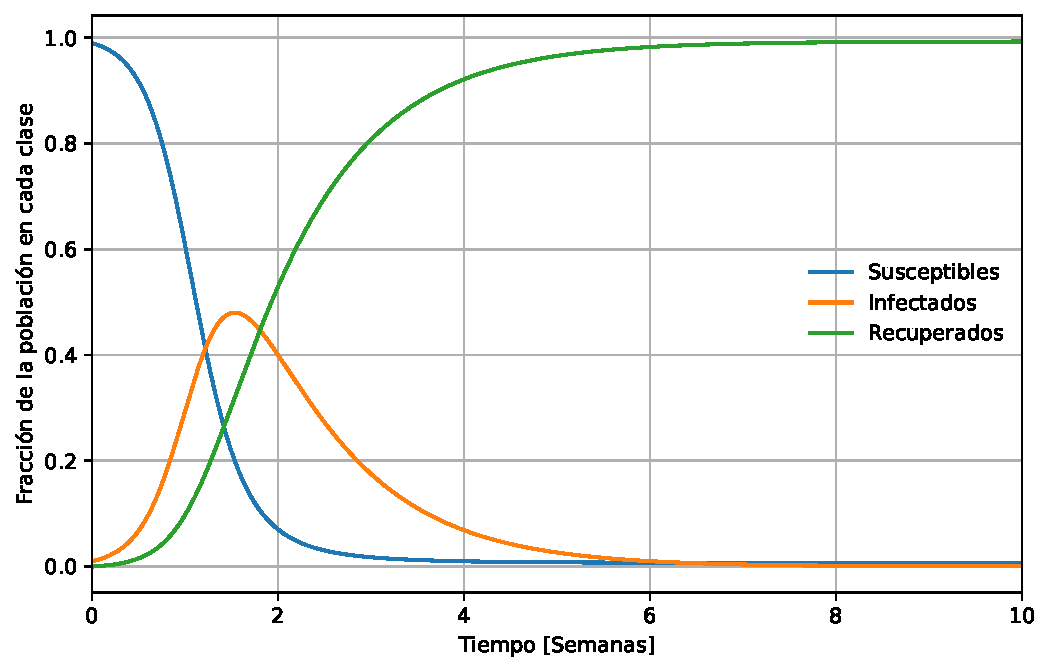
\includegraphics[width=\imsizeL]{SIR.pdf}
  \caption[Solución numérica del modelo S-I-R]{Evolución temporal de las variables del modelo resuelto numéricamente 
  con $\beta=~5$/semana, $\gamma=1$/semana, $I_0=0.01$ y $S_0=0.99$.}
  \label{fig:SIR}
\end{figure}


Es claro que la figura \ref{fig:SIR} no muestra toda la riqueza del sistema ya que simplemente muestra la solución para un solo conjunto de parámetros y 
condiciones iniciales. Es decir, es de esperar que la dinámica difiera si por ejemplo la tasa de transmisión $\beta$ es menor. En particular, es de 
interés saber para qué conjunto de parámetros $\beta$ y $\gamma$ la propagación de la infección es efectiva, es decir, si la mayoría de la población debió cursar la 
enfermedad. Esto puede determinarse de manera sencilla pidiendo que $\dv{I}{t}<0$ al momento del brote de la infección. De esto resulta que si $S_0<S_c=\gamma/\beta$ 
para cualquier $I_0>0$ entonces la infección perece y no resulta efectiva. Este es un resultado conocido obtenido por Kermack y McKendrick (1927).\cite{SIR}
El cociente $\gamma/\beta$ es la tasa de recuperación relativa, sin embargo, su recíproco le quita todos los méritos, $R_0=~\beta/\gamma$ 
conocido en epidemiología comunmente como el coeficiente de reproducción, el cual describe la media de personas infectadas por un individuo 
infectado. Dado que usualmente $S_0\approx 1$, la condición para que la infección perezca se lee ahora en función de $R_0$
simplemente como $R_0<1$. Lo cual resulta natural, si un infectado infecta en promedio a menos de una persona en lo que cursa la enfermedad entonces 
la infección no se propaga.


Es importante señalar brevemente las virtudes y fundamentalmente las hipótesis bajo las que se presenta este modelo. La ventaja más notable es la 
simplicidad y el carácter didáctico del mismo, que como vimos, permite definir y asimilar conceptos generales asociados a la problemática de manera sencilla.
Esta simplicidad, sin embargo, viene acompañada de hipótesis que en ocaciones resultan restrictivas y poco realistas en lo que respecta a una dinámica
tan compleja como lo es la propagación de una enfermedad infecciosa sobre una dada población. Por ejemplo, se ignoran efectos de demografía los cuales
pueden tener un impacto apreciable sobre la dinámica a escalas temporales extensas propias de una endemia. Además, se trata de un modelo de campo medio, 
donde se asume que cada sujeto de la población interactúa con todos los demás, es decir, desprecia hetereogeneidades que puedan surgir de la edad, el 
espacio o aspectos de comportamiento. Adicionalmente, supone que individuos que pasaron por la enfermadad adquieren inmunidad para toda la vida, que
un sujeto inmediatamente infectado puede infectar a otro y que todos los individuos infectados tienen el mismo período de infección. Por supuesto, esto 
no desmerece en nada al modelo, el cual sigue siendo extremadamente útil como primera aproximación al modelado de este tipo de sistemas complejos,
simplemente es importante recordar las hipótesis sobre las que se trabaja para evitar posibles confusiones.

Por último, es de interés mencionar que si bien el enfoque ha estado hasta ahora centrado en una descripción epidemiológica, es posible extender este 
mismo modelo de manera sencilla a otras problemáticas. En particular, puede asociarse rápidamente el modelo SIR con la dinámica
de un incendio en un bosque. Donde los <<susceptibles>> son los árboles que pueden incendiarse, los <<infectados>> son los árboles en 
llamas y los <<recuperados>> los árboles que ya han sido quemados y no pueden volver a incendiarse.


\section{Modelo SIR de reacción-difusión homogéneo}
\label{S:Modelo SIR espacial hom}

De manera general las ecuaciones de reacción-difusión sobre un medio isotrópico son aquellas que pueden escriberse como
\begin{equation}
  \pdv{\vb{u}}{t} = \vb{f} + \div(D\grad{\vb{u}}),
\end{equation}
donde $\vb{u}$ es un campo vectorial que dependende de la posición $\mathbf{x}$ y el tiempo $t$, $\vb{f}$ es el término de reacción, que es función de 
$\vb u$, $\vb x$ y $t$, mientras que $\div(D\grad{\vb{u}})$ es el término de difusión, donde D es la matriz de difusión que puede ser función de $\vb x$.
Este tipo de ecuaciones han sido ampliamente estudiadas \cite{keeling:infectious_diseases,Murray2002,Murray2003,coulson_1958} y se denominan así porque originalmente 
se utilizaron para estudiar la dinámica de reactivos químicos.\cite{turing52the}

En lo que respecta al modelo SIR de reacción-difusión que nos interesa a nosotros, este puede escribirse de manera sencilla agregando 
el término difusivo a las ecuaciones (\ref{Seq} - \ref{Req}), dejando de lado la ecuación para $R$, esto es 
\begin{align}
  \pdv{S}{t}&=-\beta SI + D_{S} \laplacian{S},\label{Seqdif}\\[.3cm]
  \pdv{I}{t}&=\beta SI - \gamma I + D_{I} \laplacian{I}.\label{Ieqdif}
\end{align}

Donde ahora $S$, $I$ y $R$ son funciones de la posición $(x,y)$ en un espacio bidimensional además del tiempo $t$, de modo que ahora 
se cumple $S(x,y,t)+I(x,y,t)+R(x,y,t)=1$ para todo $(x,y,t)$. En este nuevo modelo 
(\ref{Seqdif} - \ref{Ieqdif}) los términos difusivos dan lugar a una transmisión local de la infección. Es decir, abandonamos el modelo de campo medio que teníamos en la sección \ref{S:Modelo SIR} donde todos
los individuos podían interactuar entre sí.

Hemos supuesto que los coeficientes de difusión $D_{S}$ y $D_{I}$ son independientes de la posición y que la matriz $D$ es diagonal 
dejando de lado la posibilidad de difusión cruzada. Adicionalmente, tanto $\beta$ como $\gamma$ son 
independientes de la posición, dando lugar a un medio totalmente homogéneo, todos los puntos del espacio son equivalentes en términos de transmisión. Esta 
es una característica crítica a remarcar, ya que en la sección \ref{S:Modelo SIR espacial het} presentamos el correpondiente modelo heterogéneo, donde 
el medio puede adquirir un carácter desordenado, que es el foco de estudio de este trabajo.

A continuación se muestran algunos resultados interesantes asociados a este modelo que serán de interés a la hora de compararlo con su versión heterogénea.

\subsection{Soluciones de onda}
\label{ondas}

El objetivo principal que quiere alcanzarse es, naturalmente, el siguiente. Dada una fracción de infectados inicial $I(x,y,0)$ y una fracción de susceptibles 
distribuída homogéneamete $S(x,y,0)=S_0$, se quiere saber cómo es la evolución espacio-temporal de la fracción de infectados $I(x,y,t)$. En la problemática 
de incendios la idea sería la misma, pero cambiando infectados por, digamos, incendiados. 

Nuevamente, no es posible resolver las ecuaciones \ref{Seqdif} y \ref{Ieqdif} explícitamente, sin embargo, es posible estudiar qué condiciones deben 
satisfacerse para que cierto tipo de soluciones puedan existir. En particular, nos interesa estudiar bajo qué condiciones podría existir una solución de onda 
y qué características tendría.

Para ello proponemos una solución de onda plana donde 
\begin{align}
  S(x,y,t)&=S(z), & I(x,y,t)&=I(z), &  z&=x-ct, \label{wave}
\end{align}
que representa una onda de infección viajando en la dirección $x$ positiva con una velocidad $c>0$. Reemplazando \ref{wave} en \ref{Seqdif} y \ref{Ieqdif}, resulta el 
siguiente sistema de ecuaciones no lineales,

\begin{align}
  D_S S''+ cS'-\beta IS &=0,\label{Sz} \\[.3cm] D_I I'' + cI' + \beta I(S-\gamma/\beta)&=0, \label{Iz}
\end{align}
donde las primas indican derivadas respecto de $z$. Como es habitual, este sistema tampoco puede resolverse explícitamente, sin embargo, imponiendo las 
siguientes condiciones para las soluciones\footnote{Se utiliza la siguiente notación por simplicidad, dada una función $f(z)$, 
\[\lim_{z\to\pm\infty}f(z)\equiv f(\pm\infty)\]}
\begin{align*}
  I(\pm\infty)&=0,   &  S(\infty) &= S_0,  & S(-\infty) &= S_1,   
\end{align*}
donde $S_1$ sería la fracción de susceptibles que deja la onda por detrás, es posible linearizar la ecuación \ref{Iz} para $z$ donde $S(z)\approx S_0$,
es decir, sobre el perfil frontal de la onda. De lo cual resulta,
\begin{equation}
  D_I I'' + cI'+\beta I(S_0-\gamma/\beta)=0,\label{Idez}
\end{equation}
que tiene una solución $I(z)\propto e^{-\lambda z}$, con $\lambda$ satisfaciendo,
\[D_I \lambda^2 - c \lambda +\beta(S_0-\gamma/\beta)=0,\]
es decir,
\[\lambda = \frac{c}{2D_I}\pm \sqrt{(c/2D_I)^2-\frac{\beta}{D_I}(S_0-\gamma/\beta)}.\]
Debemos imponer además que $\lambda \in \mathds R$ con $\lambda>0$, de otra manera la solución no sería autoconsistente. Al imponer que $\lambda>0$ 
resulta $\gamma/\beta<S_0$, que es la misma condición que habíamos obtenido en la sección \ref{S:Modelo SIR} para que la infección progrese, 
mientras que ahora es una condición necesaria para la existencia de soluciones onda, las cuales darían lugar a la 
propagación de la infección, por lo menos resulta concordante. Más interesante quizás, es la condición $\lambda \in \mathds{R}$, de la cual resulta que 
\begin{align*}
  0\leq&(c/2D_I)^2-\frac{\beta}{D_I}(S_0-\gamma/\beta),\\[.3cm]
  c\geq&2\sqrt{D_I\beta(S_0-\gamma/\beta)}\equiv c_0,
\end{align*}
dando así una velocidad mínima $c_0$ para la existencia de la onda. Veremos en la sección \ref{S:aleatorios} que la velocidad de propagación es en realidad
muy cercana a la mínima encontrada aquí $c_0$. Tomando esto por cierto, el perfil frontal de la onda de infección está dado por 
\begin{equation}
  I(z)\propto \exp[-\frac{c_0}{2D_I}z].\label{larika2}  
\end{equation}

Haciendo una cuenta equivalente para el perfil posterior de la onda donde $S(z)\approx S_1$, hay que resolver la ecuación análoga a \ref{Idez}, 
$D_I I'' + cI'+\beta I(S_1-\gamma/\beta)=0$, de esto resulta 

\begin{align}
  I(z)&\propto \exp[\left(-\frac{c_0}{2D_I}+\sqrt{(c_0/2D_I)^2-\frac{\beta}{D_I}(S_1-\gamma/\beta)}\right)z], \label{larika} \\[.3cm]
  I(z)&\propto \exp[\left(-\frac{c_0}{2D_I}+ \sqrt{\frac{\beta}{D_I}(S_0-S_1)}\right)z].
\end{align}
De la ecuación \ref{larika} se ve fácilmente que es necesario que $\gamma/\beta>S_1$, de modo que en resumen se tiene la siguiente relación
\[S_0>\gamma/\beta>S_1>0,\]
es decir, que la fracción de susceptibles que quedan tras el paso de la onda no es suficiente para activar una onda de retroceso ya que $S_1<\gamma/\beta$.

En resumen, se obtuvieron expresiones analíticas aproximadas del perfil frontal y posterior que tendría una solución de onda, ecuaciones \ref{larika2} 
y \ref{larika} respectivamente, las cuales dan a entender que el perfil completo de la onda es asimétrico. Se determinó a su vez la velocidad de propagación de la onda $c_0=2\sqrt{D_I\beta(S_0-\gamma/\beta)}$ y se estableció la 
jerarquía $S_0>\gamma/\beta>S_1>0$ para la existencia de la onda.


\section{Modelo SIR de reacción-difusión heterogéneo}
\label{S:Modelo SIR espacial het}

En esta sección presentamos el modelo que estudiamos con profundidad en este trabajo junto con las descripciones estadísticas del mismo que se usarán 
luego en el capítulo \ref{Simulaciones}. 

Esencialmente las ecuaciones son las mismas que \ref{Seqdif} y \ref{Ieqdif} con la salvedad de que ahora introducimos hetereogeneidad en el medio poniendo 
una tasa de transmisión $\beta_{\vb{r}}$ dependiente de la posición. Por completitud escribimos las ecuaciones nuevamente aquí,
\begin{align}
  \pdv{S}{t}&=-\beta_{\vb{r}} SI + D_{S} \laplacian{S}  ,\label{Seqfinal}\\[.3cm]
  \pdv{I}{t}&=\beta_{\vb{r}} SI - \gamma I + D_{I} \laplacian{I}.\label{Ieqfinal}
\end{align}

Una tasa de transmisión $\beta_{\vb{r}}$ de este tipo podría utilizarse, por ejemplo, para estudiar el efecto de la vacunación sobre la población. Esto es 
entendible dado que se espera que los lugares donde hay población vacunada la tasa de transmisión sea menor ya que hay menos individuos susceptibles para
infectarse. Otra alternativa apuntaría a describir lugares donde la tasa de transmisión es más baja por un efecto de densidad poblacional. 
En cuanto a la propagación de incendios podría interpretarse de manera similar como una variación de la densidad de vegetación en el espacio, lo cual 
facilitaría o no la transmisión de las llamas.

\subsection{Problema y observables}
\label{Problema}

Vamos a centrarnos en estudiar el frente de infección/incendio en un espacio cuadrado de longitud $L$, 
con $x,y \in [0,L-1]$, y condiciones iniciales
\begin{align*}
  I(x,y,0)=&I_0, & S(x,y,0)=&1-I_0,
\end{align*}
con $x\in(0,\delta x)$ y 
\begin{align*}
  I(x,y,0)=&0, & S(x,y,0)=&S_0,
\end{align*}
para $x\in[\delta x,L-1)$. Adicionalmente, se tienen condiciones de contorno de Dirichlet en la dirección $x$,
\begin{align*}
  I(0,y,t)=I(L-1,y,t)=S(0,y,t)=S(L-1,y,t)=0. 
\end{align*}
Y condiciones periódicas en la dirección $y$, 
\begin{align*}
  I(x,0,t)=&I(x,L-1,t) & S(x,0,t)=&S(x,L-1,t). 
\end{align*}
Estas condiciones iniciales y de contorno dan lugar a un único frente de onda propagándose en la dirección $x$, lo cual resulta conveniente para realizar un análisis 
estadístico a partir de ciertos observables, los cuales se definen a continuación.

Para caracterizar las fluctuaciones espaciales y temporales del frente de infección/incendio, definimos el campo de desplazamiento del frente $u(y,t)$ como
\begin{equation}
  \max_{x\in(0,L-1)}\{I(x,y,t)\}=I(u(y,t),y,t).\label{campo}
\end{equation}
Es decir, $u(y,t)$ es la posición en $x$ del máximo de la fracción de infectados/incendiados para un dado $y$ en el instante $t$. Se define a su vez el centro de masa
de $u(y,t)$,
\begin{equation}
  u_{cm}(t)\equiv\langle u(y,t)\rangle_{y},\label{centromasa}
\end{equation}
donde $\langle...\rangle_{y}$ indica el promedio sobre la coordenada $y$. El valor medio de la amplitud máxima de $I(x,y,t)$ sobre $u(y,t)$ es,
\begin{equation}
  I_{max}(t)=\langle I(u(y,t),y,t)\rangle_{y}.\label{maximo}
\end{equation}
Por otro lado, la velocidad media de la onda de propagación se define como,
\begin{equation}
  c\equiv\langle\dot{u}_{cm}(t)\rangle_{t}.\label{velocidad}
\end{equation}
donde $\langle...\rangle_{t}$ indica promedio sobre el tiempo. De manera similar, la amplitud media del frente de propagación es
\begin{equation}
  I_{max}=\langle I_{max}(t)\rangle_{t}.  \label{Imax}
\end{equation} 
Las fluctuaciones del frente de onda pueden ser caracterizadas definiendo la rugosidad del mismo como la desviación estándar de $u(y,t)$,
\begin{equation}
  w(t)^2\equiv\langle[u(y,t)-u_{cm}(t)]^2\rangle_{y},\label{rugosidad}
\end{equation}  
o con el factor de estructura,
\begin{equation}
  S(q)\equiv\langle|u(q,t)|^2\rangle_{t},\label{factor}
\end{equation}
donde $u(q,t)$ es la transformada de Fourier sobre el espacio de $u(y,t)$.
Por último, estaremos interesados en observar el perfil de la onda de propagación, estos es,
\begin{equation}
  f_{I}(x)=\langle I(x-u(y,t),y,t)\rangle_{y,t}.\label{perfil}
\end{equation}

En el capítulo \ref{Simulaciones} utilizaremos los observables definidos aquí como principales herramientas para caracterizar y comparar de manera cuantitativa
los efectos que tienen distintas heterogeneidades, introducidas mediante $\beta_{\vb r}$, sobre la dinámica del problema. 

\subsection{Tipos de heterogeneidades}

Discutiremos aquí brevemente los distintos tipos de heterogeneidad que nos proponemos explorar en este trabajo. Para ello simplemente describimos los distintos 
$\beta_{\vb r}$ utilizados.

\subsubsection*{Heterogeneidad dicotómica-aleatoria}

El modelo (\ref{Seqfinal} - \ref{Ieqfinal}) fue estudiado por A. Kolton y K. Laneri (2019) \cite{kolton} en su trabajo sobre frentes de infección
rugosos en medios aleatorios, donde se propusieron estudiar la dínamica utlizando una tasa de transmisión $\beta_{\vb r}$ en forma de ruido dicotómico
con una distribución de probabilidad dada por 
\begin{equation}
  f(\beta_{\vb r}) = p\delta(\beta_{\vb r}) + (1-p)\delta(\beta_{\vb r}-\beta),\label{prop}
\end{equation}
donde $0\leq p \leq 1$. Esto es equivalente a decir, dada una posición $\vb r = (x,y)$, la tasa de transmisión en $\vb r$ es $0$ con probabilidad $p$ o
es $\beta$ con propabilidad $1-p$. De modo que el medio puede considerarse aleatorio. Nótese que cuando $p=0$ se recupera el caso homogéneo de la 
sección \ref{S:Modelo SIR espacial hom} donde la tasa de transmisión es $\beta$ en todo el espacio. Con la distribución de probabilidad \ref{prop}, 
este $\beta_{\vb r}$ cumple 
\begin{align}
  \overline{\beta_{\vb{r}}}&= (1-p)\beta, \\[.3cm]
  \overline{\beta_{\vb r}\beta_{\vb{r'}}} - \overline{\beta_{\vb{r}}}\;\overline{\beta_{\vb{r'}}} &= \beta^2p(1-p)\delta(\vb r - \vb{r'}),
\end{align}
donde las barras indican valor medio sobre desorden. Puede verse que no se tiene correlación espacial, por tanto se estaría representando una estrategia de vacunación 
aleatoria sobre la población. Llamaremos a la hetereogeneidad definida así como <<heterogeneidad
dicotómica-aleatoria>>.

Para ganar cierta intuición sobre lo que implica este tipo de heterogeneidad sobre el espacio, en la figura \ref{fig:heterogeneidad_dicotómica_aleatoria} 
pueden verse distintas realizaciones de $\beta_{\vb r}$ para diferentes valores de $p$ representadas sobre una grilla de $20 \times 20$.

\begin{figure}
  \centering
  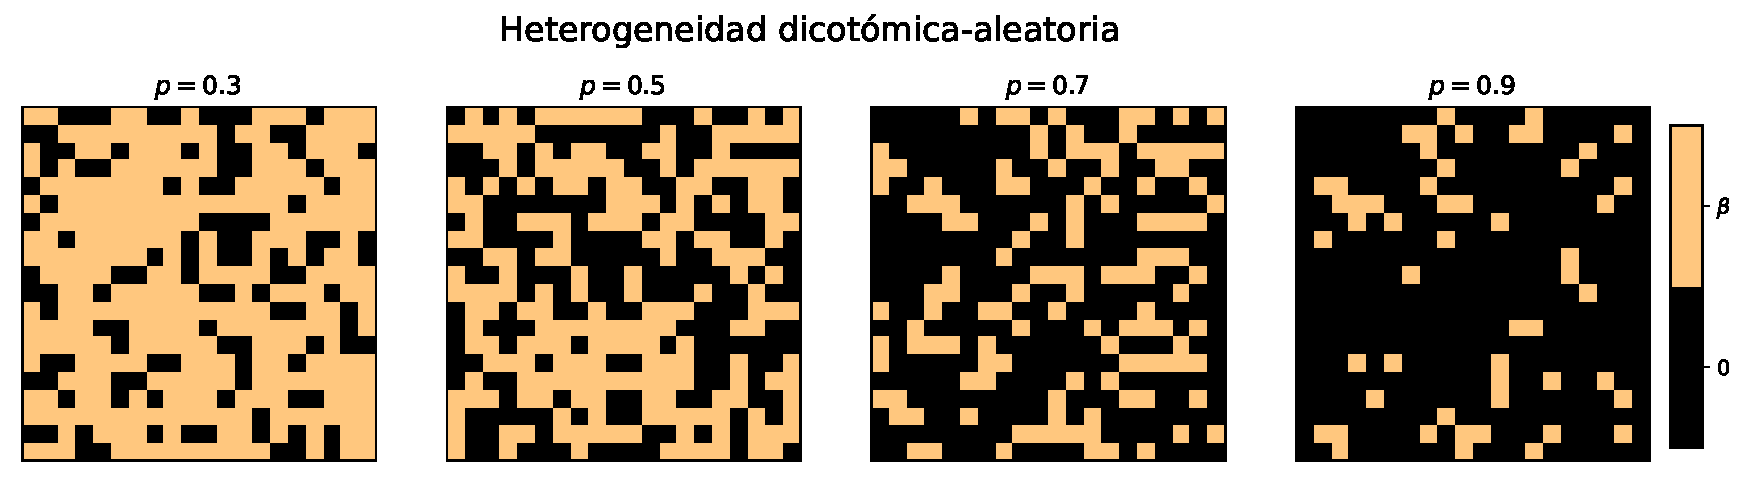
\includegraphics[width=1\textwidth]{heterogeneidad_dicot_aleatoria.pdf}
  \caption{De izquierda a derecha: representación de $\beta_{\vb r}$ sobre una grilla de $20 \times 20$ para  $p=0.3$ , $p=0.5$ , $p=0.7$ y $p=0.9$.}
  \label{fig:heterogeneidad_dicotómica_aleatoria}
\end{figure}


\subsubsection*{Heterogeneidad suavizada}

En este caso se propone una heterogeneidad suavizada, donde, en primera instancia, se genera un $\beta_{\vb r}$ usando la distribución
de probabilidad \ref{prop} y luego se aplica una regla de suavizado $n$ veces. En un esquema discreto donde el espacio de $L\times L$ se descompone en
$N\times N$ cuadrantes de $L/N$ por $L/N$, la regla de suavizado puede describirse de manera recursiva como,
\begin{align}
  \beta^{(0)}_{\vb r} &= \beta_{\vb r},\\ 
  \beta^{(n)}_{i,j} &= \frac{1}{5} (\beta^{(n-1)}_{i-1,j} + \beta^{(n-1)}_{i+1,j} + \beta^{(n-1)}_{i,j-1} + \beta^{(n-1)}_{i,j+1} + \beta^{(n-1)}_{i,j}),\label{suavizado}
\end{align}
donde $\beta^{(n)}_{i,j}$ es el valor del nuevo $\beta^{(n)}_{\vb r}$ en el cuadrante $\vb r =(i,j)$ con $i,j = 1,2...,N$.
\footnote{Se consideran condiciones periódicas sobre la grilla, de modo que por ejemplo, $i=N+1$ se entiende como $i=1$.} 

La particularidad de esta
tasa de transmisión es que ahora presenta una correlación espacial local. Esto implica que disminuirán los efectos de cambios abruptos en la tasa de 
transimisión sobre la propagación del frente de onda. Por otro lado, el valor medio $\overline{\beta^{(n)}_{\vb r}}$ es igual al valor medio 
$\overline{\beta_{\vb r}}$, esto puede verse por inducción, $\overline{\beta^{(1)}_{\vb r}}=\overline{\beta^{(0)}_{\vb r}}=\overline{\beta_{\vb r}}$,
luego, asumiendo que $\overline{\beta^{(n-1)}_{\vb r}}=\overline{\beta_{\vb r}}$ resulta que $\overline{\beta^{(n)}_{\vb r}}=\overline{\beta_{\vb r}}$.
\begin{figure}[h]
  \centering
  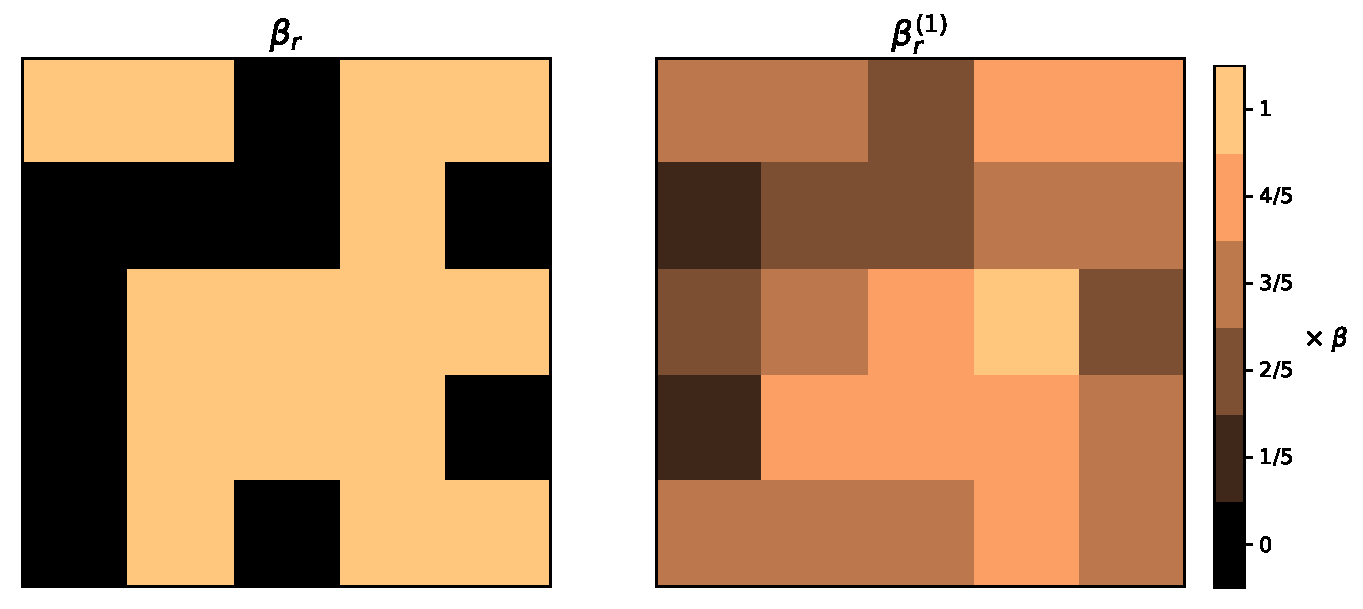
\includegraphics[width=.65\textwidth]{smoth_step.pdf}
  \caption{A la izquierda, se muestra una realización de $\beta_{\vb r}$ con $p=0.5$. A la derecha, se muestra el efecto de un paso de suavizado 
  sobre el $\beta_{\vb r}$ original.}
  \label{fig:smoth_step}
\end{figure}

En la figura \ref{fig:smoth_step} puede verse esquemáticamente el efecto de un paso de suavizado sobre una grilla de $10\times10$, mientras que 
en la figura \ref{fig:smoth} se muestran realizaciones de $\beta^{(1)}_{\vb r}$ para diferentes $p$ sobre una grilla de $20\times20$, compare con 
la figura \ref{fig:heterogeneidad_dicotómica_aleatoria}.

\begin{figure}[h]
  \centering
  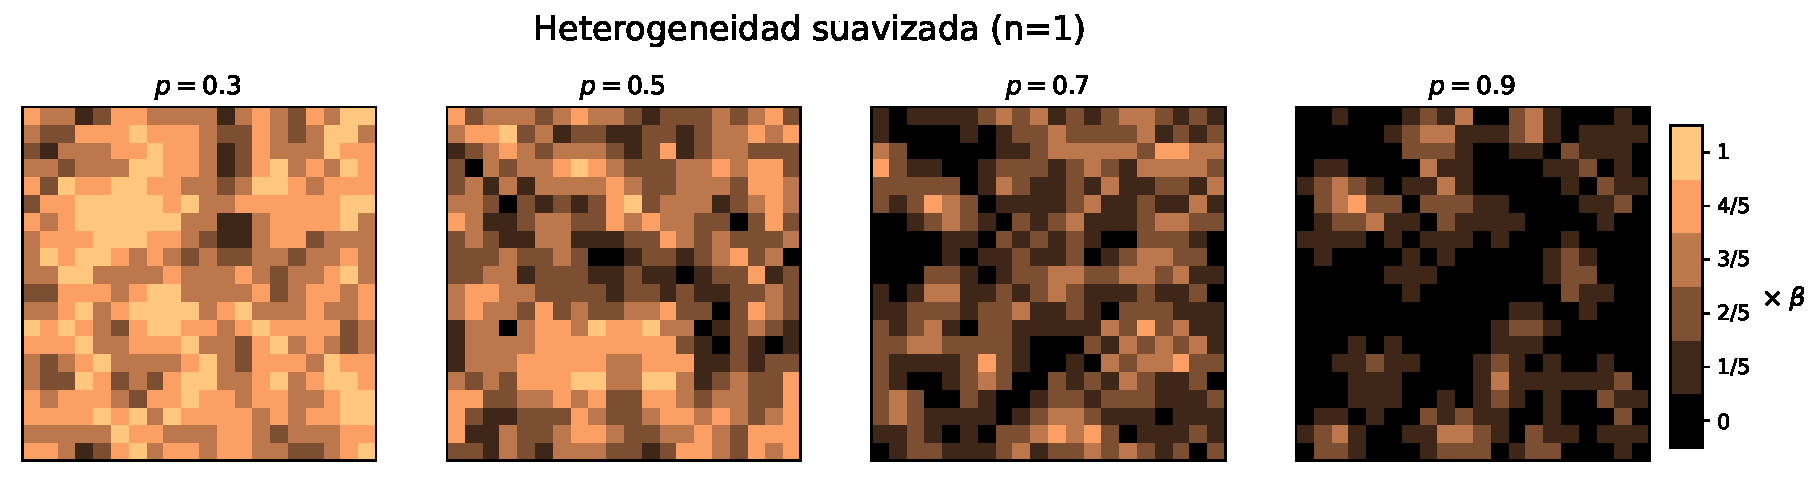
\includegraphics[width=1\textwidth]{het_suav.pdf}
  \caption{De izquierda a derecha: representación de $\beta^{(1)}_{\vb r}$ sobre una grilla de $20 \times 20$ para  $p=0.3$ , $p=0.5$ , $p=0.7$ y $p=0.9$.}
  \label{fig:smoth}
\end{figure}

Un detalle más a notar sobre este tipo de heterogeneidad es que para $n\rightarrow\infty$ recuperamos nuevamente nuevamente el caso
homogéneo de la sección \ref{S:Modelo SIR espacial hom}, con una tasa de transmisión constante en todo el espacio de valor 
$\overline{\beta_{\vb r}}=(1-p)\beta$. Esto puede verse tomando el límite en la ecuación \ref{suavizado} para $n\rightarrow\infty$, poniendo 
$\lim_{n\to \infty}\beta^{(n)}_{i,j}\equiv\beta^{(\infty)}_{i,j}$, se tiene
\[
  4\beta^{(\infty)}_{i,j} = \beta^{(\infty)}_{i-1,j} + \beta^{(\infty)}_{i+1,j} + \beta^{(\infty)}_{i,j-1} + \beta^{(\infty)}_{i,j+1},
\]
para todo $(i,j)$, de modo que la única posibilidad es que $\beta^{(\infty)}_{i,j}$ sea el mismo para todo $(i,j)$ e igual a $\overline{\beta_{\vb r}}$, ya que debe
conservar el valor medio. En la figura \ref{fig:nsmoth_step} se muestra el efecto al realizar varios pasos de suavizado.

\begin{figure}[h]
  \centering
  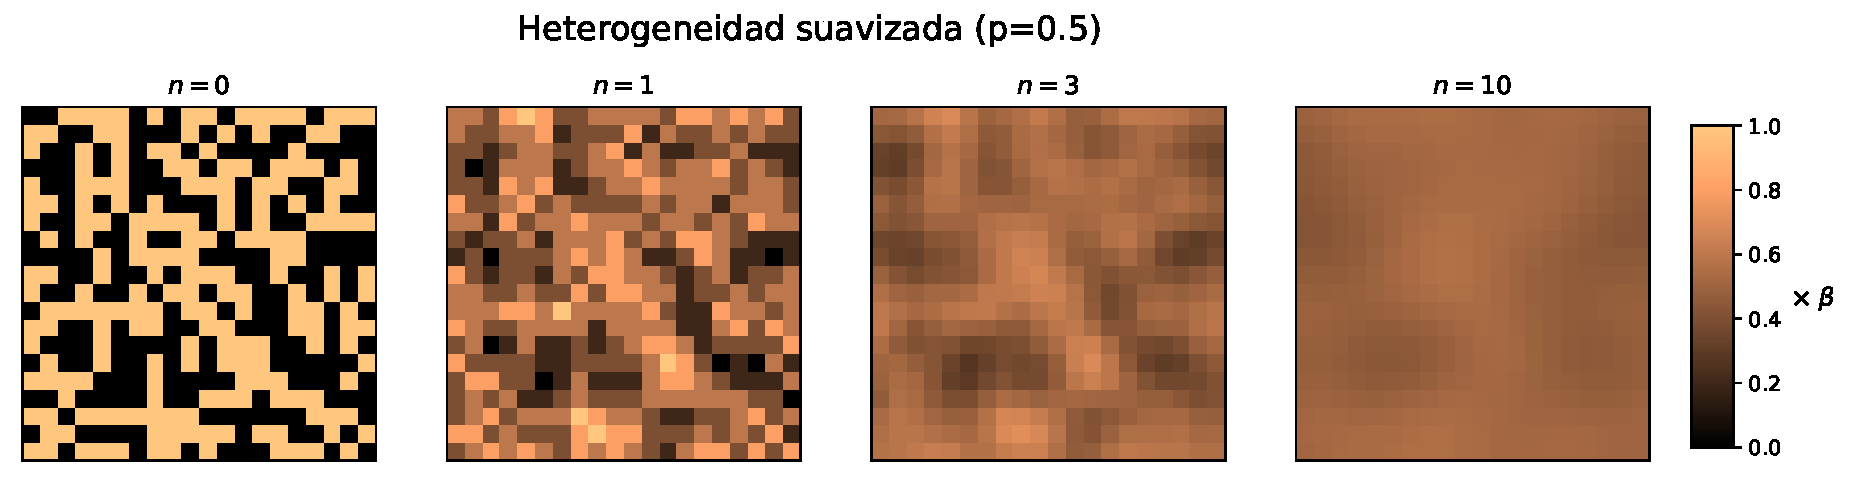
\includegraphics[width=1\textwidth]{nsmoth_step.pdf}
  \caption{De izquierda a derecha: se muestran los $\beta^{(n)}_{\vb r}$ con $n=0,1,3,10$ sobre una grilla de $20\times20$.}
  \label{fig:nsmoth_step}
\end{figure}

\subsubsection*{Heterogeneidad dicotómica-correlacionada}

Esta consiste, de alguna manera, en una combinación de las dos anteriores. Se genera un $\beta^{(n)}_{\vb r}$ de la misma manera que para la versión 
suavizada. Una vez obtenido este $\beta^{(n)}_{\vb r}$ definimos un nuevo $\tilde{\beta}^{(n)}_{i,j}$ de la siguiete manera,

\begin{align*}
  \tilde{\beta}^{(n)}_{i,j} &= \beta, \; \;\;\; \mbox{si}\; \beta^{(n)}_{i,j}\geq\overline{\beta_{\vb r}}=(1-p)\beta,  \\
  \tilde{\beta}^{(n)}_{i,j} &= 0,  \;\;\;\;\mbox{si}\; \beta^{(n)}_{i,j}<\overline{\beta_{\vb r}}=(1-p)\beta.
\end{align*}

Este caso presenta correlación local en una versión dicotómica, pero naturalmente no conserva el valor medio. En la figura \ref{fig:smoth_dic} se muestran 
realizaciones para distintos valores de $p$ con $n=1$. Puede observarse a simple viste que la densidad de puntos negros no aumenta con $p$ como 
pasaba en los casos anteriores esta diferencia sustancial en el comporamiento debe tenerse en cuenta a la hora de comparar resultados. Para ello 
utilizaremos el valor medio $\tilde{\beta}^{(n)}_{\vb r}$ en lugar de $p$, ya que da cuenta de esta variación del comportamiento.

\begin{figure}[h]
  \centering
  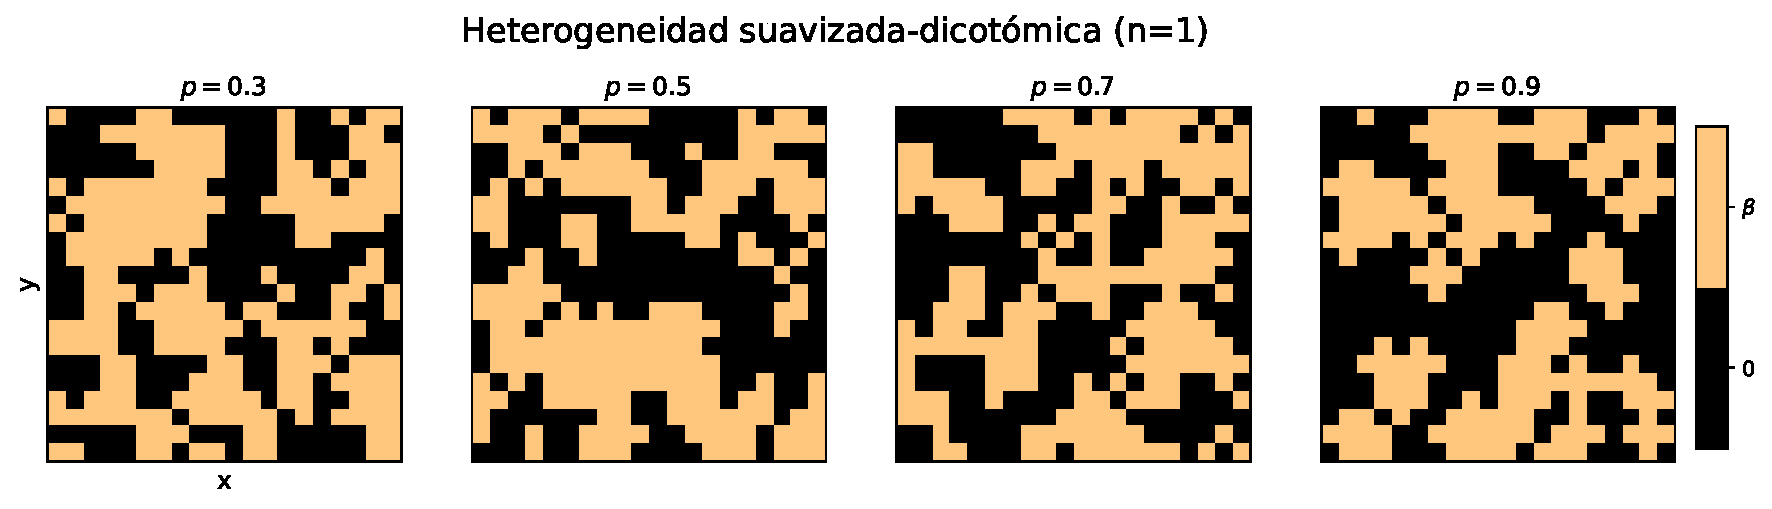
\includegraphics[width=1\textwidth]{het_suav_dico.pdf}
  \caption{De izquierda a derecha: representación de $\tilde{\beta}^{(1)}_{\vb r}$ sobre una grilla de $20 \times 20$ para  $p=0.3$ , $p=0.5$ , $p=0.7$ y $p=0.9$.}
  \label{fig:smoth_dic}  
\end{figure}

En la figura \ref{fig:smoth_dic_step} se muestra el efecto de los pasos de suavizado para este caso con $p=0.5$. En este caso, al hacer el límite 
$n\to \infty$ se recupera nuevamente el caso homogéneo pero con un valor medio de $\tilde{\beta}^{(\infty)}_{\vb r}=\beta$.

\begin{figure}[h]
  \centering
  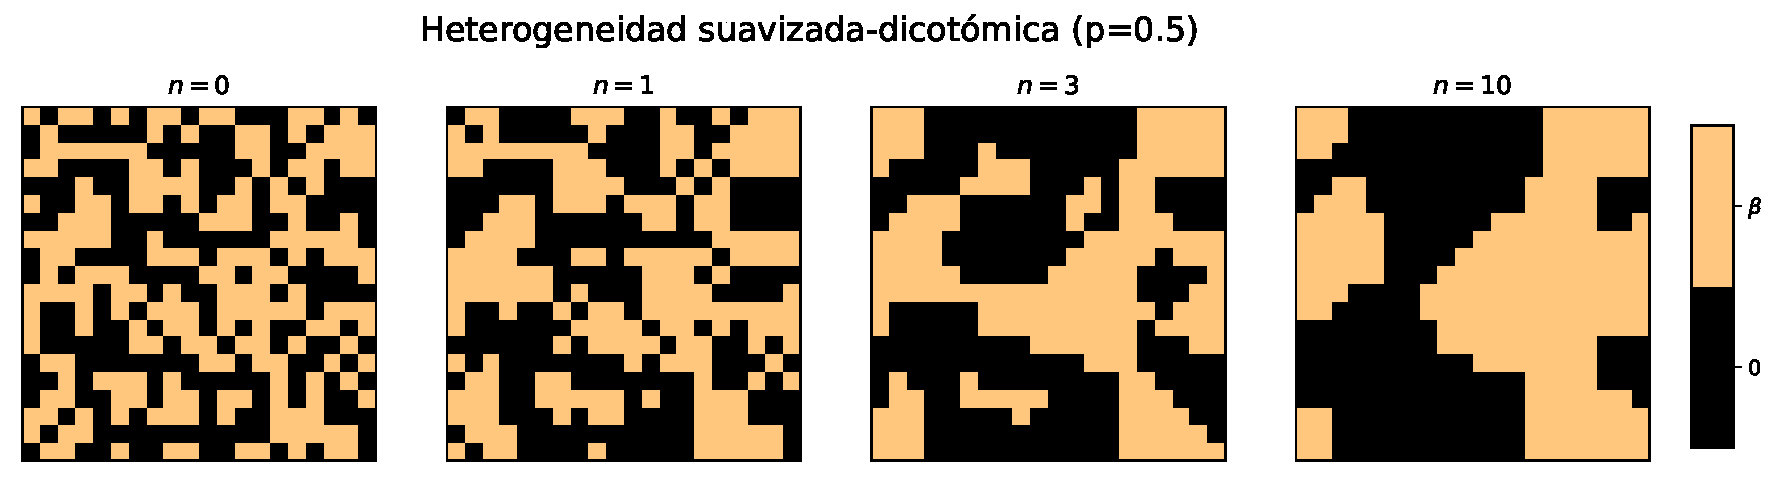
\includegraphics[width=1\textwidth]{nsmoth_dic_step.pdf}
  \caption{De izquierda a derecha: se muestran los $\tilde{\beta}^{(n)}_{\vb r}$ con $n=0,1,3,10$ sobre una grilla de $20\times20$.}
  \label{fig:smoth_dic_step}
\end{figure}